\documentclass{beamer}
\mode<presentation>
\usepackage{amsmath}
\usepackage{amssymb}
%\usepackage{advdate}
\usepackage{graphicx}
\graphicspath{{../Figs/}}
\usepackage{adjustbox}
\usepackage{subcaption}
\usepackage{enumitem}
\usepackage{multicol}
\usepackage{mathtools}
\usepackage{listings}
\usepackage{url}
\def\UrlBreaks{\do\/\do-}
\usetheme{Boadilla}
\usecolortheme{lily}
\setbeamertemplate{footline}
{
  \leavevmode%
  \hbox{%
  \begin{beamercolorbox}[wd=\paperwidth,ht=2.25ex,dp=1ex,right]{author in head/foot}%
    \insertframenumber{} / \inserttotalframenumber\hspace*{2ex} 
  \end{beamercolorbox}}%
  \vskip0pt%
}
\setbeamertemplate{navigation symbols}{}

\providecommand{\nCr}[2]{\,^{#1}C_{#2}} % nCr
\providecommand{\nPr}[2]{\,^{#1}P_{#2}} % nPr
\providecommand{\mbf}{\mathbf}
\providecommand{\pr}[1]{\ensuremath{\Pr\left(#1\right)}}
\providecommand{\qfunc}[1]{\ensuremath{Q\left(#1\right)}}
\providecommand{\sbrak}[1]{\ensuremath{{}\left[#1\right]}}
\providecommand{\lsbrak}[1]{\ensuremath{{}\left[#1\right.}}
\providecommand{\rsbrak}[1]{\ensuremath{{}\left.#1\right]}}
\providecommand{\brak}[1]{\ensuremath{\left(#1\right)}}
\providecommand{\lbrak}[1]{\ensuremath{\left(#1\right.}}
\providecommand{\rbrak}[1]{\ensuremath{\left.#1\right)}}
\providecommand{\cbrak}[1]{\ensuremath{\left\{#1\right\}}}
\providecommand{\lcbrak}[1]{\ensuremath{\left\{#1\right.}}
\providecommand{\rcbrak}[1]{\ensuremath{\left.#1\right\}}}
\theoremstyle{remark}
\newtheorem{rem}{Remark}
\newcommand{\sgn}{\mathop{\mathrm{sgn}}}
\providecommand{\abs}[1]{\left\vert#1\right\vert}
\providecommand{\res}[1]{\Res\displaylimits_{#1}} 
\providecommand{\norm}[1]{\lVert#1\rVert}
\providecommand{\mtx}[1]{\mathbf{#1}}
\providecommand{\mean}[1]{E\left[ #1 \right]}
\providecommand{\fourier}{\overset{\mathcal{F}}{ \rightleftharpoons}}
%\providecommand{\hilbert}{\overset{\mathcal{H}}{ \rightleftharpoons}}
\providecommand{\system}[1]{\overset{\mathcal{#1}}{ \longleftrightarrow}}
%\providecommand{\system}{\overset{\mathcal{H}}{ \longleftrightarrow}}
	%\newcommand{\solution}[2]{\textbf{Solution:}{#1}}
%\newcommand{\solution}{\noindent \textbf{Solution: }}
\providecommand{\dec}[2]{\ensuremath{\overset{#1}{\underset{#2}{\gtrless}}}}
\newcommand{\myvec}[1]{\ensuremath{\begin{pmatrix}#1\end{pmatrix}}}
\let\vec\mathbf

\lstset{
%language=C,
frame=single, 
breaklines=true,
columns=fullflexible
}

\numberwithin{equation}{section}


\begin{document}

\title{2.9.18}
\author{AI25BTECH11002 - Ayush Sunil Labhade}
{\let\newpage\relax\maketitle}
%\renewcommand{\thefigure}{\theenumi}
%\renewcommand{\thetable}{\theenumi}
	
\textbf{Question}:\newline

		Find the volume of a cuboid whose edges are given by  $-3\hat{\imath}+7\hat{\jmath}+5\hat{k}$,  $-5\hat{\imath}+7\hat{\jmath}-3\hat{k}$ and  $7\hat{\imath}-5\hat{\jmath}-3\hat{k}$.
		\newline
		\textbf{Solution:}
		Given:
		\begin{table}[H]
			\centering
			\begin{tabular}{|c|c|}
\hline
Point & Vector \\
\hline
$\vec{a}$ & $\myvec{3 \\ 7 \\ 5}$ \\
\hline
$\vec{b}$ & $\myvec{-5 \\ 7 \\ -3}$ \\
\hline
$\vec{c}$ & $\myvec{7 \\ -5 \\ -3}$ \\
\hline
\end{tabular}

			\label{}
			\caption{Given data}
		\end{table}
		To find volume we need to compute \sbrak{a \ b \ c}
		We will compute by finding the determinant of \sbrak{a \ b \ c}:
		\begin{align}
			\vec{D}=\myvec{a & b & c}
		\end{align}
		\begin{align}
			\vec{D} =
		\myvec{
3 & -5 & -7 \\
7 & 7 & -5 \\
5 & -3 & -3
}
		\end{align}
		On computing,
		\begin{align}
			det(\vec{D})=264
		\end{align}
		\begin{align}
			\therefore \sbrak{a \ b \ c}=264
		\end{align}
		Thus, the volume is 264.
		\newpage
		Graph:
\begin{figure}[H]
	\centering
	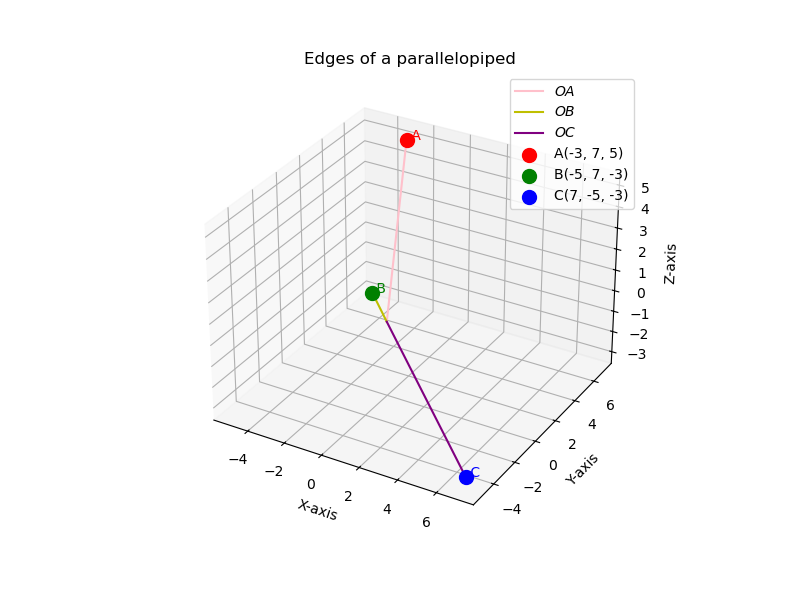
\includegraphics[scale=0.5]{plot}
	\caption*{}
	\label{fig}
\end{figure}
\end{document}
